\chapter{Simulações computacionais} \label{app:simulacoes-computacionais}
\section{Introdução}\label{sec:intro-sim-comp}
Este apêndice apresenta os principais aspectos relacionados às simulações computacionais desenvolvidas no contexto deste trabalho, com ênfase na escolha dos \textit{solvers}, no seu funcionamento e nas decisões adotadas durante a implementação dos códigos.

Na Seção~\ref{sec:app-simcomp-solvers}, discutimos os fundamentos teóricos dos \textit{solvers} utilizados, suas propriedades e os critérios que motivaram sua seleção. Em seguida, na Seção~\ref{sec:app-simcomp-consideracoes-comp}, descrevemos as decisões de implementação, dificuldades enfrentadas, soluções adotadas e observações relevantes sobre o processo de desenvolvimento computacional.

\section{\textit{Solvers}}\label{sec:app-simcomp-solvers}
Para as simulações computacionais realizadas neste trabalho, foram utilizados \textit{solvers} prontos disponíveis nas bibliotecas das linguagens de programação \textit{Python} e \textit{Julia}. De forma geral, a linguagem \textit{Python} foi empregada para a simulação de sistemas determinísticos modelados por EDOs, enquanto a linguagem \textit{Julia} foi utilizada para a modelagem de EDEs.

Nas simulações em \textit{Python}, foi adotado o método explícito de Runge-Kutta de ordem 5(4) (RK45), por meio da biblioteca \textit{SciPy}, versão 1.6.2. Já nas simulações em \textit{Julia}, utilizou-se o método de Euler-Maruyama não-rígido (EM), disponível na biblioteca \textit{SciML}, versão 7.17.0. A seguir, será apresentada uma descrição do funcionamento dos \textit{solvers} utilizados, com base nas referências disponíveis na documentação oficial das respectivas bibliotecas.


\subsection{RK45 em \textit{Python}}\label{subsec:app-simcomp-rk45-python}
O método RK45 é um método amplamente utilizado para a simulação de sistemas de EDOs. De acordo com \citet{Roma2023}, um método Runge-Kutta é definido da seguinte forma:

Um método é de \textit{Runge–Kutta explícito} de ordem $q$ se, e só se, satisfaz três propriedades:
\begin{enumerate}
	\item é um método de passo único explícito;
	\item tem as derivadas de $y(t)$ (e, portanto, de $D^j f(t,y)$) aproximadas em pontos ``convenientemente escolhidos''; e, por fim,
	\item ``concorda'' com o Método da Série de Taylor até o termo de $q$-ésima ordem, para algum $q>0$.
\end{enumerate}


Definimos um método RK explícito com $R$ estágios de forma genérica como
\begin{equation*}
	\begin{cases}
		y_0 = y(t_0),                         \\
		y_{k+1} = y_k + h\,\Phi(t_k, y_k, h), 
	\end{cases}    
\end{equation*}

onde $\Phi(t,y,h) = \sum_{r=1}^{R} c_r\,\kappa_r(t,y,h)$

Ainda segundo \citet{Roma2023}, em particular o método RK45 é definido da seguinte maneira:
\begin{equation*}
	\Phi(t,y,h)
	= \frac{25}{216}\kappa_1
	+ \frac{1408}{2565}\kappa_3
	+ \frac{2197}{4104}\kappa_4
	- \frac{1}{5}\kappa_5,
\end{equation*}

com
\begin{equation*}
	\begin{cases}
		\kappa_1 = f(t, y),                                                                                  \\
		\kappa_2 = f\bigl(t + \tfrac{h}{4},\, y + \tfrac{h}{4}\kappa_1\bigr), \                              
		\kappa_3 = f\!\left(t + \tfrac{3}{8}h,\, y + \tfrac{3}{32}h\kappa_1 + \tfrac{9}{32}h\kappa_2\right), \\
		\kappa_4 = f\!\left(t + \tfrac{12}{13}h,\, y + \tfrac{1932}{2197}h\kappa_1                           
		- \tfrac{7200}{2197}h\kappa_2 + \tfrac{7296}{2197}h\kappa_3\right),                                  \\
		\kappa_5 = f\!\left(t + h,\, y + \tfrac{439}{216}h\kappa_1                                           
		- 8h\kappa_2 + \tfrac{3680}{513}h\kappa_3                                                            
		- \tfrac{845}{4104}h\kappa_4\right).                                                                 
	\end{cases} 
\end{equation*}

O método RK45 utilizado no \textit{SciPy} possui algumas modificações que permitem uma melhor performance computacional. 

Primeiro, temos que implementa o par embutido de Dormand–Prince, proposto em \citet{Dormand1980}. 
Nesse esquema, duas fórmulas de Runge–Kutta compartilham os mesmos estágios: uma de ordem~$5$, utilizada para avançar a solução, e outra de ordem~$4$, utilizada para estimar o erro local e adaptar o passo. 

Além disso, utiliza um polinômio interpolador de ordem~4 para produzir saídas densas entre pontos consecutivos da malha, conforme descrito em \citet{Shampine1986}. Esse polinômio denso é ajustado a partir dos valores e derivadas obtidos nos extremos de cada passo, fornecendo uma aproximação contínua e suavemente diferenciável ($C^1$) da solução. Sua principal vantagem é permitir a avaliação de $y(t)$ em qualquer ponto intermediário $t \in [t_n, t_{n+1}]$ sem a necessidade de recomputar o integrador, aumentando a eficiência e a precisão da integração numérica.

\subsection{Euler-Maruyama em \textit{Julia}}\label{subsec:app-simcomp-em-julia}

O método Euler-Maruyama é um método de discretização para EDEs. Nas simulações feitas para este trabalho, ele foi selecionado pelo fato de todas as EDEs simuladas serem consideradas simples, na forma de Itô e com escala de tempo pequena.

De acordo com \cite{Kloeden1992}, para uma EDE do tipo:
\begin{equation*}
	dX_t = a(t, X_t) \,dt + b(t, X_t)dW_t 
\end{equation*}

Para $t_0 \le t \le T$, onde $t_0$ representa o tempo inicial e $T$ o tempo inicial, com valor inicial definido por: $X_{t_0} = X_0$, discretizamos o tempo da seguinte maneira:
\begin{equation*}
	t_0 = \tau_0 < \tau_1 < \tau_2 < \ldots < \tau_{N-1} < \tau_N = T
\end{equation*}

Definimos $Y_0 = X_0$ e recursivamente, definimos $Y_n+1$ como:
\begin{equation*}
	Y_{n+1} = Y_n + a(\tau_n, Y_n)(\tau_{n+1} - \tau_n) + b(\tau_n, Y_n)(W_{\tau_{n+1}} - W_{\tau_n}),
\end{equation*}
As propriedades do método apresentadas em \citet{Rackauckas2017}, são:
\begin{itemize}
	\item Ordem forte: $0.5$ (no sentido de Itô)
	\item Ordem fraca: $1.0$
	\item Intervalo de tempo: apenas intervalo de tempo fixo
	\item Tipos de ruído: todas as formas (ruído diagonal, não diagonal, escalar, aditivo e colorido)
	\item Interpretação EDE: Itô
\end{itemize}

\section{Decisões de Implementação e Observações}\label{sec:app-simcomp-consideracoes-comp}

Durante o processo de desenvolvimento das simulações computacionais, algumas escolhas se mostraram essenciais para a evolução do projeto. A seguir, apresentamos algumas considerações e observações feitas até a versão final.

\subsection{Linguagem \textit{Julia}}\label{subsec:app-simcomp-julia-lang}
A ideia inicial era utilizar exclusivamente a linguagem \textit{Julia} para as simulações computacionais. No entanto, alguns desafios surgiram ao longo do caminho. Inicialmente, os códigos foram organizados em \textit{Jupyter Notebook}s, com duas funções principais: realizar as simulações e gerar os gráficos. Contudo, essa abordagem foi descartada. O motivo principal foi que, para o exemplo simplificado descrito na seção \ref{subsec:exemplo-simplificado}, o código ultrapassava o limite de memória RAM de 16GB quando $\varepsilon = 0.1$.
    
Para contornar o problema, decidimos abandonar o uso dos arquivos \textit{Jupyter Notebook} e migramos para arquivos \textit{Julia} (\texttt{.jl}). Além disso, ao invés de realizar a simulação e a plotagem no mesmo arquivo, optamos por dividir o processo: em um arquivo, a simulação geraria um arquivo \texttt{.csv}, enquanto em outro arquivo seria feita a geração dos gráficos. Essa mudança foi crucial para o progresso do trabalho, como será detalhado nas seções seguintes.
    
Com essas alterações, o exemplo simplificado começou a funcionar, mas ainda com limitações. Quando $\varepsilon = 0.1$, o modelo falhava, e para $\varepsilon = 0.01$, a simulação não funcionava. Como o correto funcionamento para $\varepsilon = 0.01$ era essencial, decidimos testar o código em \textit{Python}, que se comportou conforme o esperado. Os outros códigos relacionados ao modelo Lorenz 80 haviam sido escritos originalmente em \textit{Python}, em um trabalho anterior que também utilizava a abordagem de \textit{Jupyter Notebook}, para o trabalho, apenas convertemos para arquivos \textit{Python} (\texttt{.py}). Assim, buscando maior consistência no trabalho, optamos por adotar o \textit{Python} como a linguagem para os sistemas determinísticos.
    
Para os sistemas estocásticos, no entanto, escolhemos continuar com \textit{Julia}. Isso se deve ao fato de que esses sistemas são mais simples e não exigem grande poder computacional. Além disso, a biblioteca \textit{Python} \textit{sdeint}, que possui \textit{solvers} para equações diferenciais estocásticas (EDE), não recebe tanta manutenção e suporte quanto a \textit{SciML} de \textit{Julia}. A \textit{SciML} não só é bem documentada, mas também conta com tutoriais em vídeo, que foram de grande ajuda ao longo do desenvolvimento.
    
\subsection{Estrutura geral dos programas de simulação}\label{subsec:app-simcomp-estrutura-geral-prog}
Todos os arquivos de simulação seguem uma estrutura padronizada. Um programa principal é responsável por executar as simulações e gerar os dados no formato \texttt{.csv}, que são armazenados na pasta \texttt{data}. Paralelamente, um segundo programa é dedicado à criação das imagens no formato \texttt{.png}, salvas na pasta \texttt{img}. Essa organização mostrou-se particularmente vantajosa pelos seguintes motivos:

\begin{enumerate}
	\item \textbf{Organização.} A separação das funcionalidades em arquivos distintos facilita a manutenção, a leitura e a modificação do código.
	\item \textbf{Desempenho.} A divisão entre simulação e visualização contribuiu para mitigar problemas de performance, conforme discutido na seção anterior.
	\item \textbf{Gerenciamento de dados.} A utilização de diretórios específicos para dados e imagens facilita o compartilhamento e está alinhada com boas práticas de gestão de arquivos em projetos computacionais.
\end{enumerate}

    
\subsection{Código-fonte das simulações BE-SLO}\label{subsec:app-simcomp-simulacoes-be-slo}
Optou-se por manter privado o código-fonte da simulação do modelo Lorenz 80 BE-SLO. Tal decisão fundamenta-se no fato de que os arquivos responsáveis pela geração dos parâmetros do modelo foram gentilmente cedidos pelo professor Honghu Liu, coautor de \citet{Chekroun2021}. Como não houve especificação explícita quanto aos direitos de uso e compartilhamento desse material, decidiu-se pela não inclusão do referido código neste relatório.
        
\subsection{Sistema integrado para diferentes versões do modelo L80}\label{subsec:app-simcomp-sis-integrado-l80}
    
Com o objetivo de facilitar a comparação entre as diferentes formulações do modelo de Lorenz 80 (PE, QG e BE), foi desenvolvido um sistema integrado que unifica a execução desses modelos em um único programa. A estrutura do código é dividida em seis módulos principais, o que favorece a organização, a manutenção e a extensibilidade do sistema:
    
\begin{enumerate}
	\item \texttt{initial\_conditions.py} – Define as condições iniciais das variáveis $x$, $y$ e $z$.
	\item \texttt{main.py} – Gerencia o fluxo de execução e a interação com o usuário, permitindo a escolha do modelo.
	\item \texttt{parameters.py} – Armazena os parâmetros utilizados nas equações e na definição das condições iniciais, centralizando valores que podem ser facilmente ajustados.
	\item \texttt{phi.py} – Implementa a função $\Phi(\mathbf{y})$, conforme definida na equação \eqref{eq:ch01-phi-be}, utilizada no modelo BE.
	\item \texttt{plot.py} – Responsável pela geração dos gráficos das soluções obtidas, permitindo a visualização dos resultados de forma automatizada.
	\item \texttt{simulations.py} – Centraliza as rotinas de simulação dos modelos PE, QG e BE, integrando o sistema de equações com os métodos numéricos definidos.
\end{enumerate}

Por fim, podemos esquematizar o funcionamento do programa da seguinte maneira:


\begin{figure}[h]
	\centering
	\resizebox{0.9\textwidth}{!}{%
		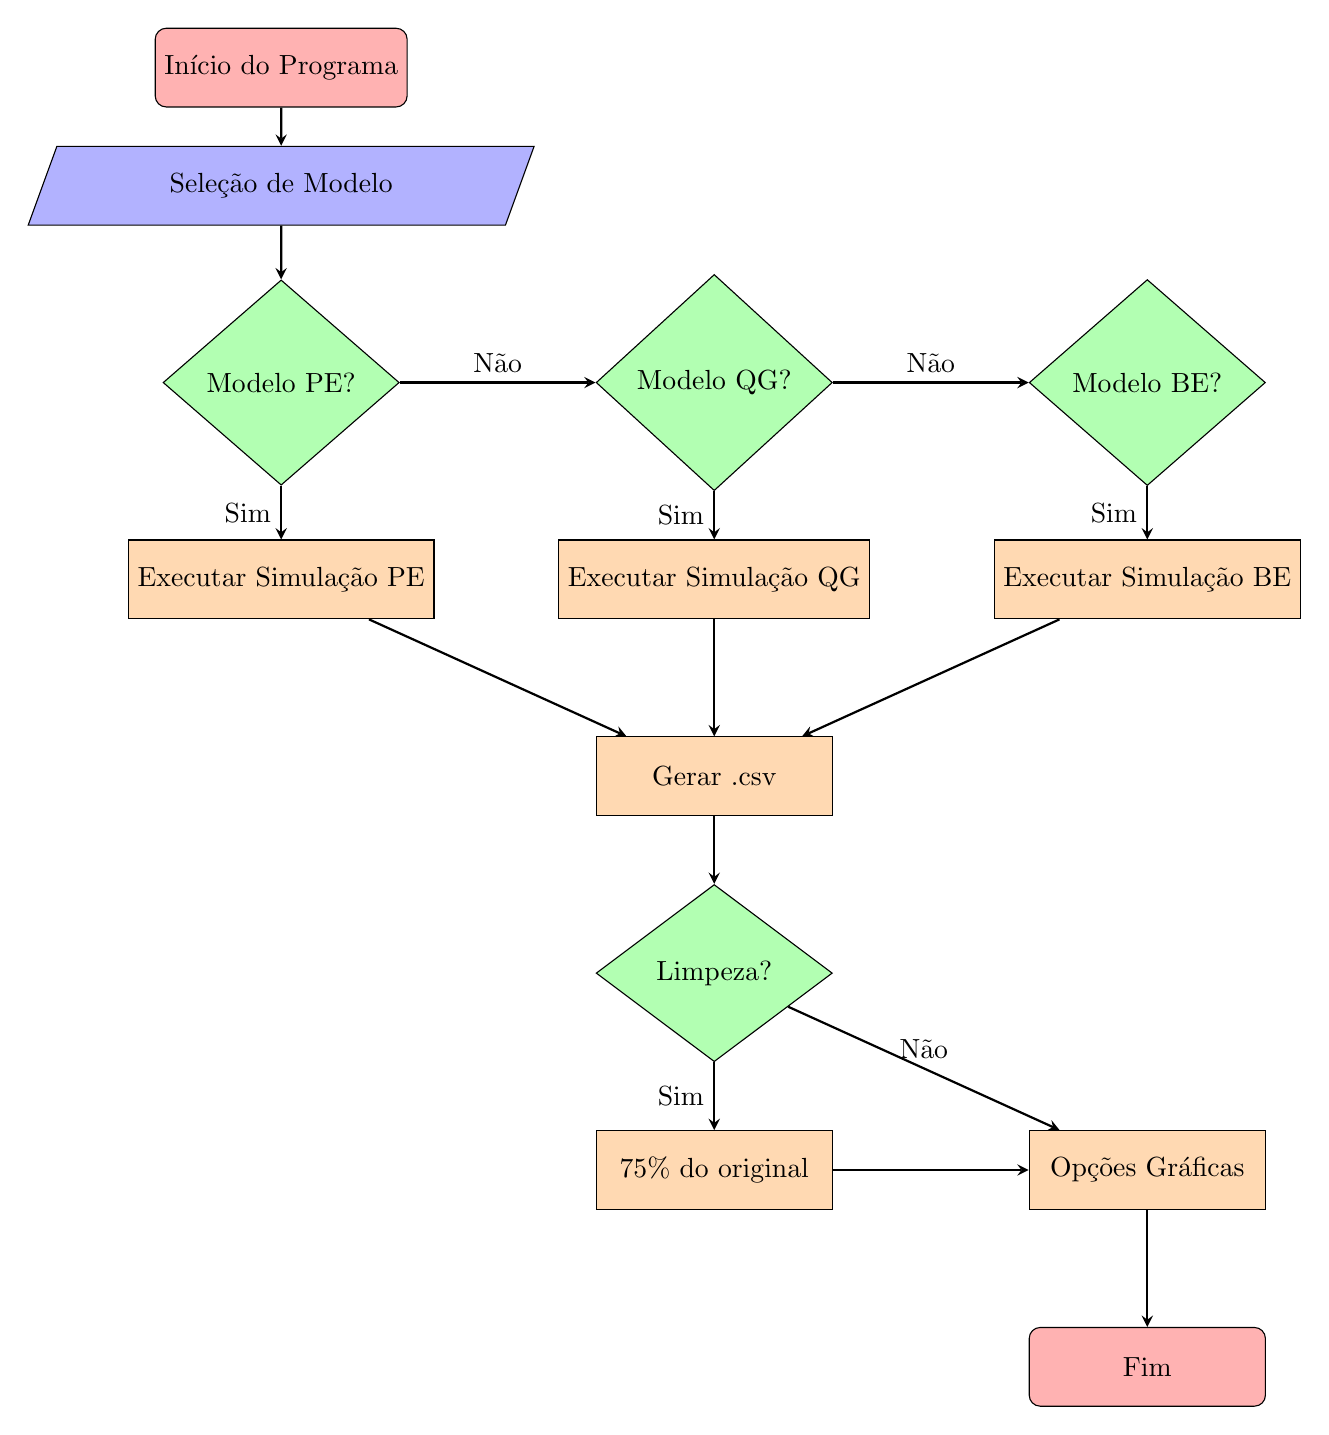
\begin{tikzpicture}[node distance=1.5cm]
			
			\usetikzlibrary{shapes.geometric, arrows}
			
			\tikzstyle{startstop} = [rectangle, rounded corners, minimum width=3cm, minimum height=1cm, text centered, draw=black, fill=red!30]
			\tikzstyle{io} = [trapezium, trapezium left angle=70, trapezium right angle=110, minimum width=3cm, minimum height=1cm, text centered, draw=black, fill=blue!30]
			\tikzstyle{process} = [rectangle, minimum width=3cm, minimum height=1cm, text centered, draw=black, fill=orange!30]
			\tikzstyle{decision} = [diamond, minimum width=3cm, minimum height=1cm, text centered, draw=black, fill=green!30]
			\tikzstyle{arrow} = [thick,->,>=stealth]
			
			% Nodes
			\node (start) [startstop] {Início do Programa};
			\node (input) [io, below of=start] {Seleção de Modelo};
			\node (decision1) [decision, below of=input, yshift=-1cm] {Modelo PE?};
			\node (decision2) [decision, right of=decision1, xshift=4cm] {Modelo QG?};
			\node (decision3) [decision, right of=decision2, xshift=4cm] {Modelo BE?};
			\node (process1) [process, below of=decision1, yshift=-1cm] {Executar Simulação PE};
			\node (process2) [process, below of=decision2, yshift=-1cm] {Executar Simulação QG};
			\node (process3) [process, below of=decision3, yshift=-1cm] {Executar Simulação BE};
			\node (process4) [process, below of=process2, yshift=-1cm] {Gerar .csv};
			\node (decision4) [decision, below of=process4, yshift=-1cm] {Limpeza?};
			\node (process6) [process, below of=decision4, yshift=-1cm] {75\% do original};
			\node (loop) [process, right of=process6, xshift=4cm] {Opções Gráficas};
			\node (end) [startstop, below of=loop, yshift=-1cm] {Fim};
			    
			% Arrows
			\draw [arrow] (start) -- (input);
			\draw [arrow] (input) -- (decision1);
			\draw [arrow] (decision1) -- node[anchor=east] {Sim} (process1);
			\draw [arrow] (decision1) -- node[anchor=south] {Não} (decision2);
			\draw [arrow] (decision2) -- node[anchor=east] {Sim} (process2);
			\draw [arrow] (decision2) -- node[anchor=south] {Não} (decision3);
			\draw [arrow] (decision3) -- node[anchor=east] {Sim} (process3);
			\draw [arrow] (process1) -- (process4);
			\draw [arrow] (process2) -- (process4);
			\draw [arrow] (process3) -- (process4);
			\draw [arrow] (process4) -- (decision4);
			\draw [arrow] (decision4) -- node[anchor=east] {Sim} (process6);
			\draw [arrow] (decision4) -- node[anchor=south] {Não} (loop);
			\draw [arrow] (process6) -- (loop);
			\draw [arrow] (loop) -- (end);
			    
		\end{tikzpicture}
	}
	\caption{Fluxograma do Processo de Simulação}
	\label{fig:app-simcomp-fluxo-sistema}
\end{figure}
